\section{Question 2}

\begin{question}
    Show that the Taylor polynomials are not great interpolating polynomials for 
    functions. Given the function $f(x) = \ln x$,
\end{question}

\subsection{Part a}

\begin{question}
    Find the first five Taylor polynomials (with no error terms) for $f(x)$ centered at $x=1$.
\end{question}

\begin{answer}
    \begin{align}
        &f(x) = \ln{(x)}\\
        &f'(x) = \tfrac{1}{x}\\
        &f''(x) = -\tfrac{1}{x^2}\\
        &f'''(x) = \tfrac{1}{x^3}\\
        &f^{(4)}(x) = -\tfrac{1}{x^4}\\
        &f^{(5)}(x) = \tfrac{1}{x^5}
    \end{align}
    The first five Taylor polynomials for $f(x)$ centered at $x = 1$ are the following:
    \begin{align}
        P_1(x) &= f(x_0) + \tfrac{f'(x_0)}{1!}(x-x_0) = 0 + \tfrac{1}{1}(x-1) = x-1\\
        P_2(x) &= f(x_0) + \tfrac{f'(x_0)}{1!}(x-x_0) + \tfrac{f''(x_0)}{2!}{(x-x_0)}^2 = x-1+\tfrac{-1}{2}{(x-1)}^2 = x-1-\frac{{(x-2)}^2}{2}\\
        P_3(x) &= f(x_0) + \tfrac{f'(x_0)}{1!}(x-x_0) + \tfrac{f''(x_0)}{2!}{(x-x_0)}^2 + \tfrac{f'''(x_0)}{3!}{(x-x_0)}^3\\
        &= x-1-\tfrac{{(x-1)}^2}{2} + \tfrac{{(x-1)}^3}{6}\\
        P_4(x) &= f(x_0) + \tfrac{f'(x_0)}{1!}(x-x_0) + \tfrac{f''(x_0)}{2!}{(x-x_0)}^2 + \tfrac{f'''(x_0)}{3!}{(x-x_0)}^3 + \tfrac{f^{(4)}}{4!}{(x-x_0)}^4\\
        &= x-1-\tfrac{{(x-1)}^2}{2} + \tfrac{{(x-1)}^3}{6} - \tfrac{{(x-1)}^4}{24}\\
        P_5(x) &= f(x_0) + \tfrac{f'(x_0)}{1!}(x-x_0) + \tfrac{f''(x_0)}{2!}{(x-x_0)}^2 + \tfrac{f'''(x_0)}{3!}{(x-x_0)}^3 + \tfrac{f^{(4)}}{4!}{(x-x_0)}^4 + \tfrac{f^{(5)}(x)}{5!}\\
        &= x-1-\tfrac{{(x-1)}^2}{2} + \tfrac{{(x-1)}^3}{6} - \tfrac{{(x-1)}^4}{24} + \tfrac{{(x-1)}^5}{120}\\
    \end{align}
\end{answer}

\subsection{Part b}

\begin{question}
    In \MATLAB, plot $f(x)$ and all five Taylor polynomials in the same plot over the interval $[.05,2]$. Use \verb+linspace(.05,2,100)+ for the interval, and plot the Taylor polynomials with dashed or dotted lines. Which polynomial fits $f(x)$ the best? Why?
\end{question}

\begin{answer}
    \begin{figure}[H]
        \centering
        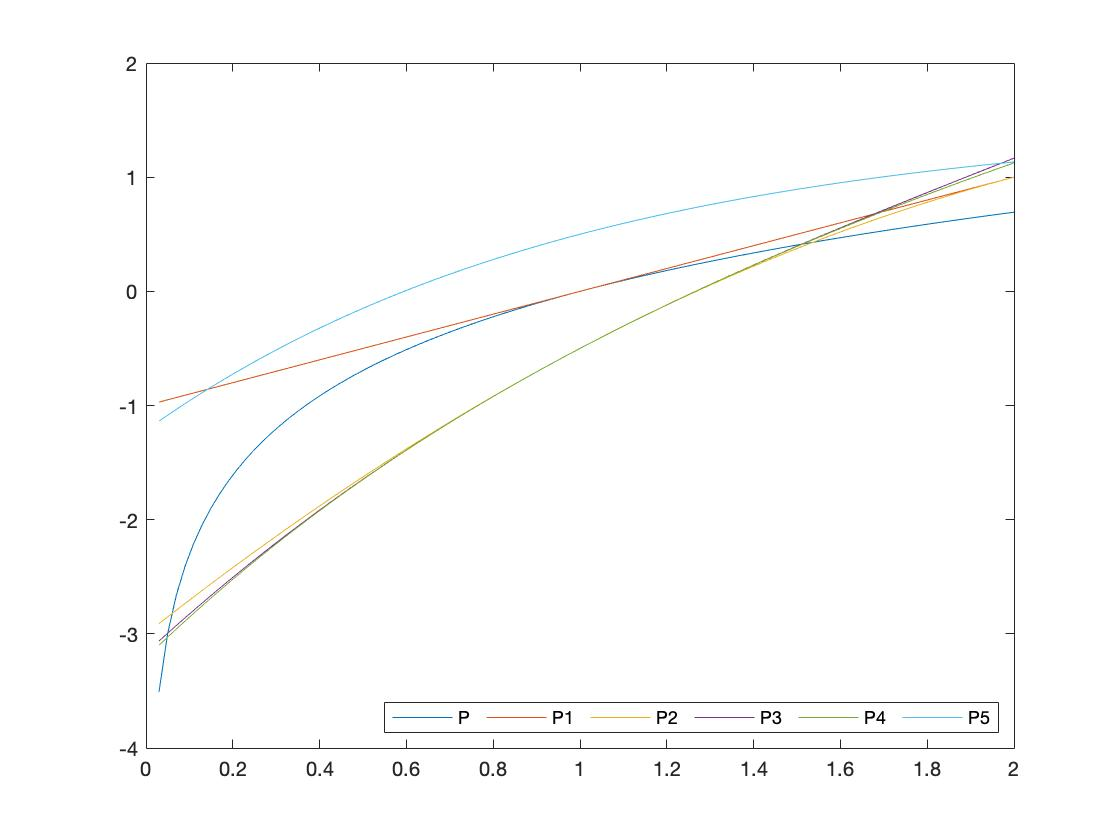
\includegraphics[width=1.0\textwidth]{Figure 3.jpg}
        \caption{\label{fig:fig3}Plot of f(x) and the Taylor polynomials over [0.05,2]}
    \end{figure}
    The plot is shown in the Figure \ref{fig:fig3}. From the plot, the first degree Taylor polynomial is the best fit for $f(x)$, since it follows the trend of the curve of the polynomial, and it gives accurate approximation around $x = 1$.
\end{answer}

\subsection{Part c}

\begin{question}
    Now, in a new figure, plot $f(x)$ and all five Taylor polynomials in the same plot over the interval $[.05,3.5]$ (Use \verb+linspace(.05,3.5,100)+ for the interval). Plot the Taylor polynomials with dashed or dotted lines. Which polynomial is the best fit for $f(x)$ now? Why?
\end{question}

\begin{answer}
    \begin{figure}[H]
        \centering
        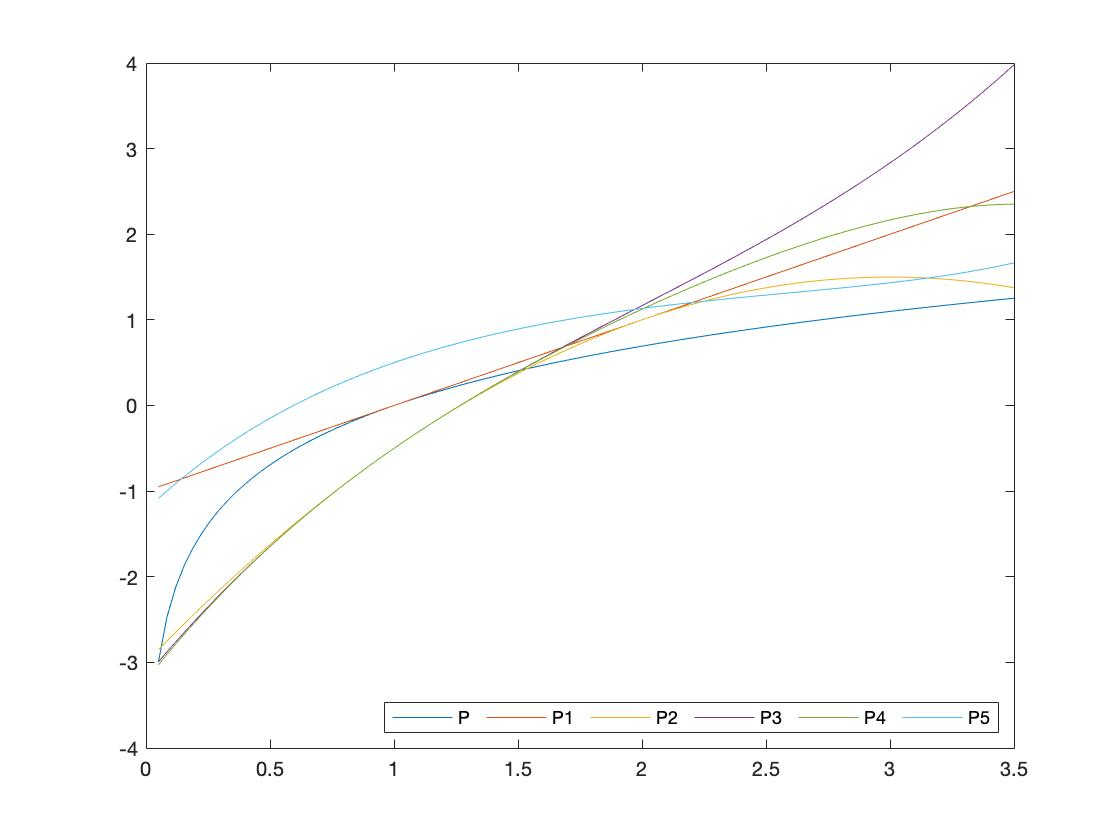
\includegraphics[width=1.0\textwidth]{Figure 4.jpg}
        \caption{\label{fig:fig4}Plot of f(x) and the Taylor polynomials over [0.05,3.5]}
    \end{figure}
    The plot is shown in the Figure \ref{fig:fig4}. Form the plot, the second degree polynomial is the best fit for $f(x)$, because as the trends in the polynomial we want to approximate, it first increases fast and then increases slowly later. Also, it is the curve the most closed to the polynomial we want to approximate.
\end{answer}